\section{\infiniteseries{Convergence Tests}}\label{conv}

It is often too difficult to determine the exact value of an infinite series (if it converges at all).  Thus, we usually settle for the knowledge \emph{that} a series converges (or diverges) as opposed to finding \emph{what} number it converges to.  By ``settling" as such, we are not actually giving up too much.  If we can guarantee that a series converges, it means it is safe to approximate it by just taking a partial sum with lots of terms.  

\begin{exercise}{Why Convergence is So Critical \Coffeecup \Coffeecup}
Why would it not make sense to approximate a divergent infinite series using a partial sum with lots of terms?
\solushun{
    If an infinite series diverges, it either goes to infinity or jumps around among various values. In the first case, an approximation doesn't make sense, and no matter how many terms we use in our partial sum, we'll never get closer than infinitely far away from infinity. In the second case, we don't get any useful information from a partial sum.\\
}{0in}
\end{exercise}

Below, we detail eight commonly used tests for convergence.

\begin{enumerate}
\item No Hope Test
\item Geometric Series Test
\item Integral Test
\item $p$ Test
\item Alternating Series Test
\item Limit Comparison Test
\item Ratio Test
\item Direct Comparison Test
\end{enumerate}

\subsection{No Hope Test and the Harmonic Series}\label{TomaytoWithMayo}
The No Hope Test is sometimes also referred to as the Divergence Test or the $n^{th}$ Term Test.  Intuitively, this test says that if the terms of the sequence $a_n$ do not go to zero, then their sum has no hope of converging.  We give a more formal statement here.

\begin{theorem}{No Hope Test}
If $\lim_{n\rightarrow \infty} a_n \not = 0$, then $\sum_{n=0}^\infty a_n$ diverges.
\end{theorem}

It does \emph{not} say the following: 
\begin{center}
\begin{align*}
\text{If }\lim_{n\rightarrow \infty} a_n  &= 0\text{, then }\sum_{n=0}^\infty a_n\text{ converges.} \tag{\Frowny}
\end{align*}
\end{center}
  This is a fallacy and a \emph{very} common mistake.  If the terms of the sequence go to zero, then the series has some chance of converging, but it is no guarantee.  Here is a classic \harmonicseries{counterexample}, the harmonic series!  The following \harmonicseries{divergence proof by Johann Bernoulli} comes from the mid-seventeenth century.

\begin{example}{Divergence of the Harmonic Series}\label{Bern}
Here we show that $$\sum_{n=0}^\infty \frac{1}{n}=\infty $$

We accomplish this by showing the partial sums will exceed any sum of one-half added to itself again and again.  Proceeding:

\begin{align*}
\sum_{n=0}^\infty \frac{1}{n}&=1+\frac{1}{2}+\frac{1}{3}+\frac{1}{4}+\frac{1}{5}+\frac{1}{6}+\frac{1}{7}+\frac{1}{8}+\frac{1}{9}+\frac{1}{10}+\frac{1}{11}+\frac{1}{12}+\frac{1}{13}+\frac{1}{14}+\frac{1}{15}+\frac{1}{16}+\cdots \\
&>1+\frac{1}{2}+\frac{1}{4}+\frac{1}{4}+\frac{1}{8}+\frac{1}{8}+\frac{1}{8}+\frac{1}{8}+\frac{1}{16}+\frac{1}{16}+\frac{1}{16}+\frac{1}{16}+\frac{1}{16}+\frac{1}{16}+\frac{1}{16}+\frac{1}{16}+\cdots \\
&=1+\frac{1}{2}+\frac{2}{4}+\frac{4}{8}+\frac{8}{16}+\cdots \\
&=1+\frac{1}{2}+\frac{1}{2}+\frac{1}{2}+\frac{1}{2}+\cdots \\
&=\infty
\end{align*}
Since the harmonic series is greater than a sum of one-half added to itself infinitely many times, it is infinite.
\end{example}

\begin{exercise}{Justifying the Steps \Coffeecup \Coffeecup}
Annotate the above proof with a short comment justifying each line of equality or inequality.
    \solushun{
    \begin{align*}
        \sum_{n=0}^\infty \frac{1}{n}&=1+\frac{1}{2}+\frac{1}{3}+\frac{1}{4}+\frac{1}{5}+\frac{1}{6}+\frac{1}{7}+\frac{1}{8}+\frac{1}{9}+\frac{1}{10}+\frac{1}{11}+\frac{1}{12}+\frac{1}{13}+\frac{1}{14}+\frac{1}{15}+\frac{1}{16}+\cdots \\
        &\text{The first line simply writes out the harmonic series.}\\
        &>1+\frac{1}{2}+\frac{1}{4}+\frac{1}{4}+\frac{1}{8}+\frac{1}{8}+\frac{1}{8}+\frac{1}{8}+\frac{1}{16}+\frac{1}{16}+\frac{1}{16}+\frac{1}{16}+\frac{1}{16}+\frac{1}{16}+\frac{1}{16}+\frac{1}{16}+\cdots \\
        &\text{We replace terms between reciprocal powers of two so that we can set up sums to one-half.}\\
        &=1+\frac{1}{2}+\frac{2}{4}+\frac{4}{8}+\frac{8}{16}+\cdots \\
        &\text{We consolidate the terms, summing terms with like denominators.}\\
        &=1+\frac{1}{2}+\frac{1}{2}+\frac{1}{2}+\frac{1}{2}+\cdots \\
        &\text{Reducing the fractions from the previous step, we get a series of $\frac{1}{2}$.}\\
        &=\infty\\
        &\text{Summing a positive constant infinitely many times gives $\infty$.}
    \end{align*}
    }{0in}
\end{exercise}

\begin{exercise}{Revisiting a Convergent Series \Coffeecup \Coffeecup \Coffeecup}
In the previous section, we showed that $$\frac{1}{2}+\frac{1}{4}+\frac{1}{8}+\frac{1}{16}+\cdots=1.$$
If you attempt to use Bernoulli's argument to show that it diverges, where does it break down?  Why can't you just group terms together into batches that are at least size one-half?
    \solushun{
        The first one-half would come from the first term itself.  But since the total is one, it means the terms $\frac{1}{4}+\frac{1}{8}+\frac{1}{16}+\cdots$ must themselves total to be the other one-half.  Thus, we can try to group terms to form batches that total to one-half, but the second batch uses up all infinitely many remaining terms! \\
    }{.5in}
\AnswerKeyEntry{The first one-half would come from the first term itself.  But since the total is one, it means the terms $\frac{1}{4}+\frac{1}{8}+\frac{1}{16}+\cdots$ must themselves total to be the other one-half.  Thus, we can try to group terms to form batches that total to one-half, but the second batch uses up all infinitely many remaining terms! }
\end{exercise}

\begin{exercise}{No Hope Test Backwards \Coffeecup}
Explain why the Harmonic Series is a counterexample to the claim tagged with \Frowny.  
    \solushun{
        For the Harmonic Series, $a_n=\frac{1}{n}$ and $\lim_{n\to\infty}\frac{1}{n}=0$. However, $\sum_n^\infty a_n = \infty$, and is thus divergent.\\
    }{.5in}
\end{exercise}

\begin{example}{Where NHT Applies and Does Not Apply}
\begin{itemize}
\item Consider the infinite series $$ \sum_{n=0}^\infty \arctan(n). $$  We notice that $\lim_{n\to \infty}\arctan(n)=\pi/2\neq 0$.  Thus, the series diverges by NHT, since we are essentially adding up infinitely many copies of $\pi/2$ to itself.
\item Consider the infinite series $$ \sum_{n=0}^\infty \arctan\left(\frac{1}{n}\right).$$  Since $\lim_{n\to \infty}\arctan\left(\frac{1}{n}\right)=0$, we cannot make any conclusion about this series via NHT.  The summand approaches zero, so there is some hope of the series converging, but further work would be required to determine this.
\end{itemize}
\end{example}
Now try a few on your own!

\begin{exercise}{Practice with the No Hope Test \Coffeecup \Coffeecup}
\begin{itemize}
\item Use the No Hope Test to prove that the series $ \sum_{n=1}^\infty \frac{\sqrt{2n^2+2}}{n}$ diverges.
    \solushun{
        Take the limit $\lim_{n\to\infty}\frac{\sqrt{2n^2+2}}{n}$. We need to use LHR and a trick:
        \begin{align*}
            \lim_{n\to\infty}\frac{\sqrt{2n^2+2}}{n}&=\lim_{n\to\infty}\sqrt{\frac{2n^2+2}{n^2}}\\
            &=\sqrt{\lim_{n\to\infty}\frac{2n^2+2}{n^2}}\\
            &=\sqrt{\lim_{n\to\infty}\frac{4n}{2n}}\\
            &=\sqrt{2}.
        \end{align*}
        Since the limit is greater than 0, we can say the series diverges.\\
    }{.5in}
\item Use the No Hope Test to prove that the series $ \sum_{n=1}^\infty \cos(1/n)$ diverges.
    \solushun{
        Evaluate $\lim_{n\to\infty}\cos\left(\frac{1}{n}\right)$:
        \begin{align*}
            \lim_{n\to\infty}\cos\left(\frac{1}{n}\right) &= \cos(0) = 1.
        \end{align*}
        Since the limit is greater than 0, we know the limit diverges.\\
    }{.5in}
\item What does the No Hope Test tell you about the convergence/divergence of the series $ \sum_{n=1}^\infty \sin(1/n)$?  
    \solushun{
        Since $\lim_{n\to\infty}\sin\left(\frac{1}{n}\right)=\sin(0) = 0$, the No Hope Test gives us no information about the convergence or divergence of $\sin\left(\frac{1}{n}\right)$.\\
    }{.5in}
\end{itemize}
\AnswerKeyEntry{The first two summands have limits of $\sqrt{2}$ and 1, respectively.  Since these limits are nonzero, the series has no hope of converging and thus diverges.  The third summand does approach zero as $n$ goes to infinity, so it gives no information.}
\end{exercise}

\subsection{\geometricseries{Geometric Series Test}}
This is essentially just a restatement of the main result of Subsection \ref{Geometrickery}, the Geometric Series Formula.  Recall that a geometric series is a series of the form $$ \sum_{n=0}^\infty a\cdot r^n$$ for some real numbers $a$ and $r$.  That is to say, it is a series that has starting term $a$ and common ratio $r$.
\begin{theorem}{Geometric Series Test}
A geometric series converges if $|r|<1$ (and in fact converges to the value $a/(1-r)$) and diverges otherwise.
\end{theorem}

\begin{exercise}{Practice with the Geometric Series \Coffeecup \Coffeecup \Coffeecup}
\begin{itemize}
\item Explain why $\sum_{n=1}^\infty \frac{1}{n^2}$ is not a geometric series (and thus this test would be inapplicable).
    \solushun{
        The summation $\sum_{n=1}^\infty \frac{1}{n^2}$ has no common ratio $r$. The first three terms are $1, \frac{1}{4}, \frac{1}{9}$, which have no ratio in commin.\\
    }{.5in}
\item Explain why the series $18-6+2-\frac{2}{3}+\frac{2}{9}-\cdots$ converges absolutely.
    \solushun{
        The common ratio is $r=-\frac{1}{3}$. Since $|r|<1$, this series converges by the Geometric Series Test. If we take the absolute value of each term in the series, we get $18+6+2+\frac{2}{3}+\frac{2}{9}+\cdots$, which has the same common ratio and thus also converges. Thus, the series converges absolutely.\\
    }{.5in}
\item Give an example of a geometric series that converges conditionally, or explain why it is not possible to construct such a series.
    \solushun{
        It is not possible to build a conditionally convergent geometric series, because the determining factor in whether a geometric series converges or not is whether $|r| >1$. So, taking the absolute value of each term in the series might flip the sign of the ratio, but it would not change the magnitude. So, any convergent geometric series must converge absolutely.\\
    }{.5in}
\end{itemize}
\AnswerKeyEntry{\textbullet The summation $\Sigma_{n=1}^\infty \frac{1}{n^2}$ has no common ratio $r$ and thus is not a geometric series. For example, the first three terms are $1,1/4,$ and $1/9$.  Thus, the first two ratios between consecutive terms are $1/4$ and $4/9$, which are not equal.  \textbullet The given geometric series has common ratio $r=-1/3$.  After taking the absolute value of each term, it becomes the series $18+6+2+\frac{2}{3}+\frac{2}{9}+\cdots$ which still converges as it now has common ratio $r=1/3$.  \textbullet It is not possible to build a conditionally convergent geometric series.  If we are given a convergent geometric series, then the common ratio $r$ satisfies $|r|<1$.  Taking the absolute value of each term in the series might flip the sign on $r$, but it will not change the magnitude.  Thus, any convergent geometric series must converge absolutely.}
\end{exercise}

\begin{exercise}{Why Not Arithmetic? \Coffeecup \Coffeecup \Coffeecup}
Why is there \emph{not} another result in this section called the ``\arithmeticseries{Arithmetic Series Test}''?  Why is only the geometric series getting to have all the fun?
    \solushun{
        Since an arithmetic series has a common difference, the sum will always be growing, either towards infinity or negative infinity. This is because we will always be adding progressively larger terms to the sum, or progressively more negative terms. But we will never add terms that get smaller and smaller in magnitude. Thus, in an arithmetic series, the sum will never converge.\\
    }{.5in}
\end{exercise}

\subsection{Integral Test}\label{IntTest}

Here we use integrals to \integ{test convergence of infinite series}!  Intuitively this test says the following:

\begin{center}
\emph{An infinite series converges if and only if the corresponding improper integral converges.} 
\end{center}

\begin{theorem}{Integral Test}

Let $a\in \mathbb{N}$ and $f(n)$ be a decreasing function on $\left[ a,\infty\right)$.  If $\int_{x=a}^{x=\infty} f(x) \dif x$ converges, then $\sum_{n=a}^\infty f(n)$ converges as well.  Conversely, if $\int_{x=a}^{x=\infty} f(x) \dif x$ diverges, then $\sum_{n=a}^\infty f(n)$ diverges as well.  

\end{theorem}

Here is a ``proof by picture'' to \area{justify the Integral Test}.

\begin{exercise}{Explaining the Integral Test \Coffeecup \Coffeecup \Coffeecup}
Study the following diagrams and use them to determine why the series converges if and only if the series converges.  Specifically:


\begin{itemize}
\item Explain why the diagram below justifies the inequality $$\int_{x=a}^{x=\infty} f(x)\dif x\leq \sum_{n=a}^\infty f(n).  $$
    
    \begin{center}
		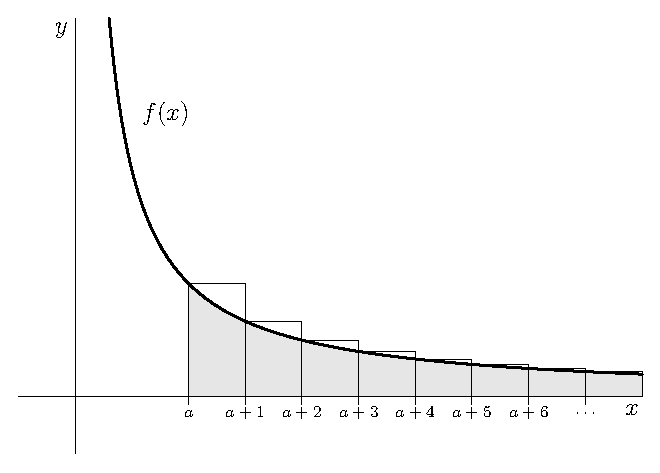
\includegraphics[width=300pt]{ChapterSeqSer/Figures/inttest2.eps}
	\end{center}


\vspace*{1in}
\item Explain why the diagram below justifies the inequality $$ \sum_{n=a+1}^\infty f(n)\leq  \int_{x=a}^{x=\infty} f(x)\dif x.  $$

	\begin{center}
		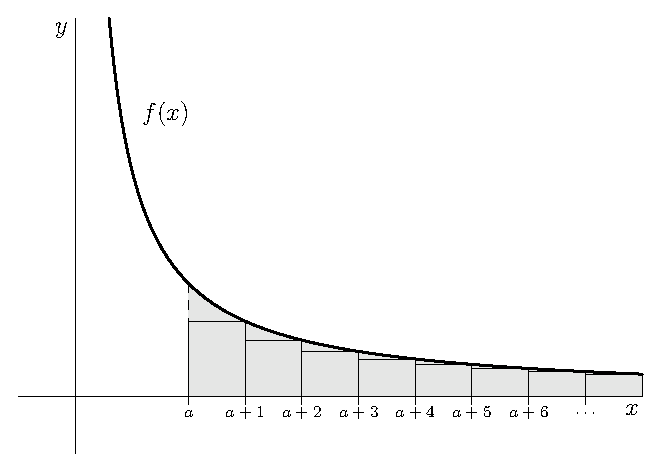
\includegraphics[width=300pt]{ChapterSeqSer/Figures/inttest1.eps}
	\end{center}
    
\vspace*{1in}
\item Add $f(a)$ to both sides of the previous inequality to conclude $$ \sum_{n=a}^\infty f(n)\leq  f(a)+\int_{x=a}^{x=\infty} f(x)\dif x.  $$

\vspace*{.5in}

\item Putting both inequalities together, we now have that \begin{align*}
\int_{x=a}^{x=\infty} f(x)\dif x \leq \sum_{n=a}^\infty f(n)\leq  f(a)+\int_{x=a}^{x=\infty} f(x)\dif x. \tag{$\bowtie $}
\end{align*} 
Explain why this inequality shows that the infinite series converges if and only if the corresponding improper integral converges.

\vspace*{.5in}

\end{itemize}
\end{exercise}

\begin{example}{Using the Integral Test}\label{UsingIntTest}
\begin{itemize}
\item The infinite series $\sum_{n=1}^\infty \frac{1}{n^2}$ converges because the corresponding improper integral is \begin{align*}
\int_{x=1}^{x=\infty}\frac{1}{x^2}\dif x &=\lim_{c\to\infty}\left.-\frac{1}{x}\right]_{x=1}^{x=c}\\
&=\lim_{c\to\infty}-\frac{1}{c}--\frac{1}{1}\\
&=1.
\end{align*}  Since the improper integral converges to a finite value, the Integral Test says that the corresponding infinite series converges as well.
\item The infinite series $\sum_{n=1}^\infty \frac{1}{\sqrt{n}}$ diverges because the corresponding improper integral is \begin{align*}
\int_{x=1}^{x=\infty}\frac{1}{\sqrt{x}}\dif x &=\lim_{c\to\infty}\left.2\sqrt{x}\right]_{x=1}^{x=c}\\
&=\lim_{c\to\infty}2\sqrt{c}-2\sqrt{1}\\
&=\infty.
\end{align*}  Since the improper integral diverges, the Integral Test says that the corresponding infinite series diverges as well.
\end{itemize}
\end{example}

\begin{exercise}{Practice with the Integral Test \Coffeecup \Coffeecup }
Use the Integral Test to decide if the following infinite series converge or diverge.
\begin{itemize}
\item $\sum_{n=2}^\infty \frac{1}{n\mathtt{ln}(n)}$
\vspace*{1in}
\item  $\sum_{n=2}^\infty \frac{1}{n(\mathtt{ln}(n))^2}$
\vspace*{1in}
\item  $\sum_{n=2}^\infty \frac{1}{n^2+1}$
\vspace*{1in}
\end{itemize}
\end{exercise}

The next example shows why the assumption of $f(x)$ being a decreasing function is necessary for the Integral Test.  

\begin{exercise}{An Interesting Example \Coffeecup \Coffeecup \Coffeecup}
Consider the function $$f(x)=\left|\sin(\pi x)\right| $$
\begin{itemize}
\item Graph the function $f(x)$ over the positive $x$-axis.
\vspace*{1in}
\item Explain why the integral $\int_{x=0}^{x=\infty} f(x)\dif x$ is equal to infinity.
\vspace*{1in}
\item Compute the infinite sum $ \sum_{n=0}^\infty f(n)$.
\vspace*{1in}
\item In this case, the integral diverged, while the infinite sum converged.  Why does this example not contradict the Integral Test?
\vspace*{.5in}
\end{itemize}
\end{exercise}

\subsection{$p$-Test}
The next result is just a special case of the Integral Test.  However, it comes up often enough that it is worth stating on its own.

\begin{theorem}{The $p$-Test }
Let $p$ be a real number.  Then the sum $\sum_{n=1}^\infty \frac{1}{n^p}$ converges for $p>1$ and diverges otherwise. 
\end{theorem}

\begin{exercise}{Justifying the $p$-Test Using the Integral Test \Coffeecup }
\begin{itemize}
\item Apply the Integral Test to the series $\sum_{n=1}^\infty \frac{1}{n^p}$ in the case where $p>1$.  Show the corresponding improper integral converges, and thus the series does as well.
\vspace*{1in}
\item Apply the Integral Test to the series $\sum_{n=1}^\infty \frac{1}{n^p}$ in the case where $p<1$.  Show the corresponding improper integral diverges, and thus the series does as well.
\vspace*{1in}
\item What does the series $\sum_{n=1}^\infty \frac{1}{n^p}$ do when $p=1$? 
\vspace*{1in}
\end{itemize}
\AnswerKeyEntry{For $p>1$ or $p<1$, one can repeat the corresponding calculations from Example \ref{IntTest}.\ref{UsingIntTest}.  If $p=1$, the series is the harmonic series, which diverges.}
\end{exercise}

\subsection{\alternatingseries{Alternating Series Test and Error Bound}}

\begin{theorem}{Alternating Series Test (AST)}
Let $a_n$ be a decreasing sequence of positive numbers that approaches zero as $n$ approaches infinity.  The summation $$\sum_{n=0}^\infty \left(-1\right)^n a_n $$ converges. 
\end{theorem}
Intuitively, this test says that the positives and negatives will cancel each other out and the partial sum pendulum will eventually stabilize at some well-defined limit. 

\begin{example}{Using AST}
Consider the series $\sum_{n=0}^{\infty} \left(-\frac{1}{2}\right)^n$.  This series can be rewritten as $\sum_{n=0}^{\infty} \left(-1\right)^n\left(\frac{1}{2}\right)^n$.  Since the sequence $\left(\frac{1}{2}\right)^n$ is positive and decreasing to zero, AST tells us that it converges. 
\end{example}
\begin{exercise}{Conditional vs Absolute \Coffeecup}
Did the above series converge conditionally or absolutely?  Explain. \vspace*{.3in}
\AnswerKeyEntry{Taking term-by-term absolute values produces the series $1+\frac{1}{2}+\frac{1}{4}+\frac{1}{8}+\cdots=2$.  Since it totals to a finite value, the original series converges absolutely.}
\end{exercise}
Notice that the above series also converges by the Geometric Series Test.  It is very common that more than one convergence test will apply to the same series.
\begin{exercise}{Tests Not Applying \Coffeecup}

\begin{itemize}
\item Explain why the convergence of $\sum_{n=0}^{\infty} \left(-\frac{1}{2}\right)^n$ cannot be analyzed using the No Hope Test. 
\vspace*{.5in}
\item Explain why the convergence of $\sum_{n=0}^{\infty} \left(-\frac{1}{2}\right)^n$ cannot be analyzed using the Integral Test. 
\vspace*{.5in}
\item Explain why the convergence of $\sum_{n=0}^{\infty} \left(-\frac{1}{2}\right)^n$ cannot be analyzed using the $p$-Test.
\vspace*{.5in}
\AnswerKeyEntry{\textbullet Since $\lim_{n\to\infty}\left(-\frac{1}{2}\right)^n=0$, the No Hope Test gives no information. \textbullet The Integral Test does not apply since the terms are not positive and decreasing.  In this case, it is actually even worse than that, as the function $\left(-\frac{1}{2}\right)^x$ is undefined for all half-integer values of $x$. \textbullet The summand is not of the form $1/n^p$, so the very narrow $p$-Test does not apply.}
\end{itemize}

\end{exercise}
\begin{exercise}{The AST in Action \Coffeecup \Coffeecup}
For each of the series below, explain why it converges by AST or explain why AST does not apply to that series.
\begin{itemize}
\item $\sum_{n=2}^\infty \frac{(-1)^n}{\ln(n)}$
\vspace*{1in}
\item  $\sum_{n=1}^\infty \frac{\cos(\pi n)}{n}$
\vspace*{1in}
\item  $\sum_{n=1}^\infty \left(\pi/2-\arctan(n)\right)^n$
\vspace*{1in}
\item  $\sum_{n=1}^\infty \left(\arctan(n)-\pi/2\right)^n$
\vspace*{1in}

\end{itemize} \AnswerKeyEntry{The first two and last converge by AST.  It does not apply to the third.}
\end{exercise}

In a convergent \errorbounds{alternating series}, the partial sums always ``leapfrog'' back and forth over the limiting value the series converges to.  This implies that the value of the infinite series is always no further away than the next unused term in any partial sum.

\begin{center}
	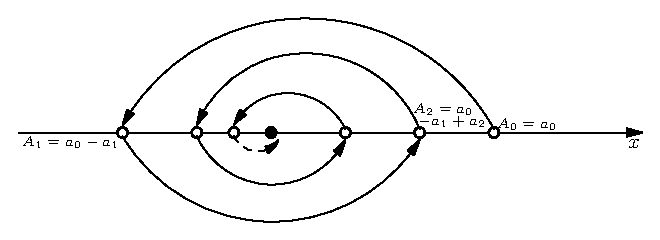
\includegraphics{ChapterSeqSer/Figures/CAS}
\end{center}

\begin{theorem}{Alternating Series \alternatingseries{Error Bound}}
Let $a_n$ be a sequence of positive decreasing terms.  Let $\sum_{n=0}^\infty (-1)^na_n$ be a convergent series.  Then the error in a partial sum is always less than the first unused term in that partial sum.  That is, $$\left|\sum_{n=0}^\infty (-1)^na_n - \sum_{n=0}^N (-1)^na_n\right|<|a_{N+1}|. $$
\end{theorem}

\begin{example}{Alternating Series Error Bug}
Consider again the bug described in Exercise \ref{infser}.\ref{alternatebug}.  Suppose we wish to know how close the bug is to its ending destination after it has reversed course two times.  Since the series is a convergent alternating series, we can use the Alternating Series Error Bound to determine how close it is to its final location.  In particular, the Alternating Series Error Bound implies $$\left|\left(\frac{1}{2}-\frac{1}{4}+\frac{1}{8}-\frac{1}{16}+\cdots\right)-\left(\frac{1}{2}-\frac{1}{4}+\frac{1}{8}\right)\right|<\frac{1}{16}. $$ 

To independently verify this claim, notice that we had already concluded in Exercise \ref{infser}.\ref{alternatebug} that the infinite series totaled to $\frac{1}{3}$.  If we plug in this value, we obtain \begin{align*}
\left|\left(\frac{1}{3}\right)-\left(\frac{1}{2}-\frac{1}{4}+\frac{1}{8}\right)\right|&=\left|\frac{1}{3}-\left(\frac{3}{8}\right)\right|\\   
&=\left|\frac{8}{24}-\frac{9}{24}\right|\\
&=\left|-\frac{1}{24}\right|
\end{align*}
which is indeed less than one-sixteenth.
\end{example}

\begin{exercise}{Alternating Series Error Bug \Coffeecup \Coffeecup} 
\begin{itemize}
\item  After the bug has reversed course three times, how close does the Alternating Series Error Bound guarantee the bug is to its final location? 
\vspace*{1in}
\item How many times would the bug have to reverse course for the Alternating Series Error Bound to guarantee the bug is within one one-thousandth of its final location?  After you figure this out, compute the corresponding partial sum and verify that it is within $0.001$ of one-third.
\vspace*{1in}
\end{itemize} \AnswerKeyEntry{After three reversals, the bug is within $\frac{1}{32}$ of its final location.  The bug would have to reverse course nine times to be guaranteed by the Alternating Series Error Bound to be within one one-thousandth of its final location. }
\end{exercise}

\subsection{Limit Comparison Test}\label{LCTomato}

This test says that if two sequences have the same growth order, then the corresponding infinite series either both converge or both diverge.  This works because if two sequences have the same growth order, then in the long term they are just a nonzero constant factor apart, and multiplying by a nonzero constant factor cannot change convergence or divergence.  Furthermore, having larger magnitude terms than a divergent series implies divergence, and smaller magnitude terms than a convergent series implies convergence.

\begin{theorem}{Limit Comparison Test (\growthorder{LCT})}
Let $a_n$ and $b_n$ be sequences of nonnegative terms. 
\begin{itemize}
\item Suppose $a_n$ has larger growth order than $b_n$, and $\sum_{n=0}^\infty b_n$ diverges.  Then $\sum_{n=0}^\infty a_n$ also diverges.
\item Suppose $a_n$ has smaller growth order than $b_n$, and $\sum_{n=0}^\infty b_n$ converges.  Then $\sum_{n=0}^\infty a_n$ also converges.
\item Suppose $a_n$ and $b_n$ have the same growth order.  Then $\sum_{n=0}^\infty a_n$ and $\sum_{n=0}^\infty b_n$ either both converge or both diverge.
\end{itemize}
\end{theorem}


A short intuitive way to state LCT is as follows: \begin{center}
\emph{A series with smaller growth order than a convergent series must also be convergent.  A series with larger growth order than a divergent series must also be divergent.}
\end{center}

The Limit Comparison Test is particularly useful if $a_n$ is expressed as a fraction with the numerator and denominator both algebraic (expressed just with polynomials and radicals).  In this case, one can build a comparison sequence by taking the ratio of leading terms from the numerator and denominator.

\begin{example}{Using Leading Terms from the Numerator and Denominator}
Suppose we wish to determine the convergence/divergence of  $$\sum_{n=1}^\infty  \frac{7n+3}{n\sqrt{n^2+n+1}}.$$
Call the summand $a_n=\frac{7n+3}{n\sqrt{n^2+n+1}}$.  The idea is that in the numerator, the ``plus three'' is insignificant as $n$ approaches infinity.  Thus, we keep only the $7n$ in the numerator.  In the denominator, we observe that the $n+1$ is insignificant compared to the $n^2$ it is being added to.  Again, we keep only the $n\sqrt{n^2}=n\cdot n = n^2$, the leading term of the denominator.  We have built our comparison function $$b_n=\frac{7n}{n^2}=\frac{7}{n}.$$  Sometimes it is nice to visualize this as just crossing out all lower order terms.  For large $n$, 

$$\frac{7n+\bcancel{3}}{n\sqrt{n^2+\bcancel{n}+\bcancel{1}}}\approx\frac{7n}{n^2}=\frac{7}{n}. $$

Next, we verify that $a_n$ and $b_n$ have the same growth order.  Proceeding with the limit, we have

\begin{align*}
\lim_{n \rightarrow \infty}\frac{a_n}{b_n}&=\lim_{n \rightarrow \infty}\frac{7n+3}{n\sqrt{n^2+n+1}}\frac{n}{7} \\
&=\lim_{n \rightarrow \infty}\frac{7n+3}{7\sqrt{n^2+n+1}} \\
&=\lim_{n \rightarrow \infty}\frac{7n^2+3n}{7n\sqrt{n^2+n+1}} \\
&=\lim_{n \rightarrow \infty}\frac{7n^2+3n}{7\sqrt{n^2}\sqrt{n^2+n+1}} \\
&=\lim_{n \rightarrow \infty}\frac{7n^2+3n}{7\sqrt{n^4+n^3+n^2}} \\
&=\lim_{n \rightarrow \infty}\frac{7n^2+3n}{7\sqrt{n^4+n^3+n^2}}\frac{\frac{1}{n^2}}{\frac{1}{\sqrt{n^4}}} \\
&=\lim_{n \rightarrow \infty}\frac{7+\frac{3}{n}}{7\sqrt{1+\frac{1}{n}+\frac{1}{n^2}}} \\
&=\frac{7}{7\sqrt{1}}\\
&=1.
\end{align*}

Thus, $a_n$ and $b_n$ have the same growth order, since their ratio is a nonzero constant. Furthermore, $$\sum_{n=1}^\infty \frac{7}{n}=7\sum_{n=1}^\infty \frac{1}{n}$$ which diverges by Bernoulli's argument in Example \ref{TomaytoWithMayo}.\ref{Bern}.   By LCT, $\sum_{n=1}^\infty  \frac{7n+3}{n\sqrt{n^2+n+1}}$ diverges as well.
\end{example}

\begin{exercise}{Practice with LCT}
Use LCT to determine whether the series converge or diverge.
\begin{itemize}
\item $\sum_{n=1}^\infty \frac{n+2}{n^3+1}$
\vspace*{2in}
\item  $\sum_{n=1}^\infty \frac{n^5}{n\sqrt{n^7+3n+1}}$
\vspace*{2in} 
\end{itemize} \AnswerKeyEntry{The first converges by comparison to $\Sigma \frac{1}{n^2}$.  The second diverges by comparison to $\Sigma \frac{1}{n^{-1/2}}$.}
\end{exercise}

Note that one can attempt to apply LCT can be applied to essentially any  function, not just algebraic functions.  However, when transcendental functions are involved, it can be more difficult to identify choice of comparison function.

\begin{example}{Cosine of Reciprocals}\label{rabbit}
Consider the series $\sum_{n=1}^\infty \left(1-\cos\left(\frac{1}{n}\right)\right)$. 
We admittedly pull a rabbit out of a hat and decide to compare to the series $\sum_{n=1}^\infty\frac{1}{n^2}$.  We demonstrate the summands have the same growth order by taking a limit of their ratios.  In particular,
\begin{align*}
\lim_{n\to\infty}\frac{1/n^2}{1-\cos\left(\frac{1}{n}\right)}&=\lim_{n\to\infty}\frac{-2/n^3}{\sin\left(\frac{1}{n}\right)\left(-1/n^2\right)} \\
&=\lim_{n\to\infty}\frac{2/n}{\sin\left(\frac{1}{n}\right)} \\
&=\lim_{n\to\infty}\frac{-2/n^2}{\cos\left(\frac{1}{n}\right)\left(-1/n^2\right)} \\
&=\lim_{n\to\infty}\frac{-2}{\cos\left(\frac{1}{n}\right)} \\
&=\lim_{n\to\infty}\frac{2}{\cos\left(\frac{1}{n}\right)} \\
&=\frac{2}{1}\\
&=2.
\end{align*}
Since the limit is a nonzero constant, we conclude that $\frac{1}{n^2}$ and $\left(1-\cos\left(\frac{1}{n}\right)\right)$ have the same growth order.  Since the series $\sum_{n=1}^\infty\frac{1}{n^2}$ converges, we use LCT to conclude that $\sum_{n=1}^\infty \left(1-\cos\left(\frac{1}{n}\right)\right)$ also converges. 
\end{example}
The above example may be a bit unsatisfying in the sense that we gave no indication where the choice of comparison function came from.  Hang in there though!  Once we have techniques of power series in our toolbox, we will revisit such examples and see why this was in fact a very natural choice of comparison.
\begin{exercise}{In and Out of L'Hospital \Coffeecup}
\begin{itemize}
\item In the above example, LHR was applied twice.  Identify which two lines it was used on.  In each case, make a brief note as to why it was valid to use LHR.  
\item In the above example, we compared to the series $\sum_{n=1}^\infty\frac{1}{n^2}$.  How did we know that series was convergent?
\vspace*{.2in}
\end{itemize}
\end{exercise}
\begin{exercise}{Sine of Reciprocals \Coffeecup \Coffeecup \Coffeecup}
Determine the convergence or divergence of the series $\sum_{n=1}^\infty \sin\left(\frac{1}{n}\right)$.

\vspace*{1.5in}

\AnswerKeyEntry{Use the comparison function $\frac{1}{n}$ to show the series diverges.}
\end{exercise}
\subsection{Ratio Test}

This test is essentially a LCT against a geometric series.

\begin{exercise}{Ratio of Consecutive Terms \Coffeecup}
If $a_n$ is a geometric sequence, what is $a_{n+1}/a_n$?
\vspace*{.5in}
\end{exercise}

For a sequence that is not geometric, there may not be a constant ratio of consecutive terms, but we can still look at the \ratiotest{limit of ratios of successive terms}!

\begin{theorem}{Ratio Test}
Consider the series $$\sum_{n=0}^\infty a_n. $$
\begin{itemize}
\item If $\lim_{n\rightarrow \infty}\left\lvert a_{n+1}/a_n \right\rvert <1$ then the series converges absolutely.
\item If $\lim_{n\rightarrow \infty}\left\lvert a_{n+1}/a_n>1 \right\rvert$ then the series diverges.
\item If $\lim_{n\rightarrow \infty}\left\lvert a_{n+1}/a_n=1 \right\rvert$ then the ratio test gives no information.
\end{itemize}
\end{theorem}

The Ratio Test is particularly helpful in analyzing series involving factorials, since so much cancellation will occur when computing the ratio of consecutive terms.

\begin{example}{A Series with Factorials \Coffeecup \Coffeecup}
Here we analyze the convergence of the series $$\sum_{n=0}^\infty \frac{2^n}{n!}. $$

Call $a_n=\frac{2^n}{n!}$.  We now compute the limit of the ratio of consecutive terms.  Proceeding, we have

\begin{align*}
\lim_{n\rightarrow \infty} \frac{a_{n+1}}{a_n}&=\lim_{n\rightarrow \infty} \frac{\frac{2^{(n+1)}}{(n+1)!}}{\frac{2^n}{n!}}\\
&=\lim_{n\rightarrow \infty} \frac{2^{(n+1)}}{2^n}\frac{n!}{(n+1)!}\\
&=\lim_{n\rightarrow \infty} 2\frac{n\cdots 3 \cdot 2 \cdot 1 }{(n+1)\cdot n \cdots 3 \cdot 2 \cdot 1 } \\
&=\lim_{n\rightarrow \infty} \frac{2}{n+1}\\
&=0 \\
&<1.
\end{align*}
Thus, the series converges by the Ratio Test!  
\end{example}

\begin{exercise}{Practice with Ratio Test \Coffeecup \Coffeecup}
Use the Ratio Test to prove the following series converge or diverge, or explain why the Ratio Test provides no information in that case.
\begin{itemize}
\item $\sum_{n=1}^\infty \frac{n+1}{n!}$
\vspace*{1.5in}
\item  $\sum_{n=1}^\infty \frac{1}{1+n^2}$
\vspace*{1.5in} 
\item  $\sum_{n=1}^\infty \frac{n!}{(2n)!}$
\vspace*{1.5in} 
\item  $\sum_{n=1}^\infty \frac{2^n}{n^{10}}$
\vspace*{1.5in}
\end{itemize}
\AnswerKeyEntry{\textbullet Converges, ratio 0. \textbullet No info, ratio 1. \textbullet Converges, ratio 0. \textbullet Diverges, ratio 2.}
\end{exercise}

\subsection{Direct Comparison Test}

The Direct Comparison Test (DCT) is similar to LCT, except we are directly comparing magnitudes of terms instead of growth orders.  We already used the idea of DCT in both Bernoulli's analysis of the Harmonic series and the Integral Test. 

\begin{theorem}{Direct Comparison Test}

Let $a_n$ and $b_n$ be sequences.  If for all natural numbers $n$, $|a_n|\leq |b_n|$, then

\begin{itemize}

\item $\sum_{n=0}^\infty b_n$ converges implies that $\sum_{n=0}^\infty a_n$ also converges. 

\item $\sum_{n=0}^\infty a_n$ diverges implies that $\sum_{n=0}^\infty b_n$ also diverges. 
\end{itemize}
\end{theorem}

A short intuitive way to state DCT is as follows: \begin{center}
\emph{A series smaller than a convergent series must also be convergent.  A series larger than a divergent series must also be divergent.}
\end{center}

The trick when using DCT is to pick an easy series to compare to, for example a $p$-series.  

\begin{example}{Redirect the Trig Function}
Here we analyze the convergence of the series $\sum_{n=1}^\infty \frac{1}{n\left(3+\sin(n)\right)}. $  Notice that $-1<\sin(n)<1 $ for all $n\in\mathbb{N}$.  Adding three to all sides of that inequality produces $$ 2<3+\sin(n)<4.$$  Thus, we can bound our summand as $$ \frac{1}{n\left(4\right)}<\frac{1}{n\left(3+\sin(n)\right)}<\frac{1}{n\left(2\right)}.$$
The right-hand side bound gives no information, but on the left-hand side we have something useful!  In particular, the series $\sum_{n=1}^\infty\frac{1}{4n}=\frac{1}{4}\sum_{n=1}^\infty\frac{1}{n}=\infty$.  Since our series in question is larger than a series that totals to infinity, it must also diverge to infinity.
\end{example}

\begin{exercise}{Practice with DCT \Coffeecup \Coffeecup}

Use the Direct Comparison Test to prove the following series converge or diverge.

\begin{itemize}

\item $\sum_{n=1}^\infty \frac{\cos(n)}{n^2}$

\vspace*{1.5in}

\item  $\sum_{n=1}^\infty \frac{2+\cos(n)}{n}$

\vspace*{1.5in} 

\item  $\sum_{n=1}^\infty \frac{1}{n^2+1}$

\vspace*{1.5in} 
\end{itemize}
\AnswerKeyEntry{These series are convergent by DCT against $\frac{1}{n^2}$, divergent by DCT against $\frac{1}{n}$, and convergent by DCT against $\frac{1}{n^2}$.}
\end{exercise}

\subsection{Mixed Practice with Convergence Tests}
In practice, when you encounter a series, there are usually many tests that will apply.  Try the following, using any valid applicable test you like!

\begin{exercise}{Mixed Practice \Coffeecup \Coffeecup \Coffeecup}
Determine if each of the following infinite series converges absolutely, converges conditionally, or diverges.  In each case, explain what tests you used and how!

\begin{itemize}

\item $\sum_{n=0}^{\infty} \frac{n}{n+2} $

\vspace*{1.5in}

\item $\sum_{n=0}^{\infty} \frac{n}{n^2+2}$

\vspace*{1.5in}

\item $\sum_{n=0}^{\infty} \frac{(-1)^nn}{n^2+2}$

\vspace*{1.5in}

\item $\sum_{n=0}^{\infty} \frac{(-1)^nn}{n^3+2}$

\vspace*{1.5in}

\end{itemize} \AnswerKeyEntry{\textbullet Divergent by NHT or Integral Test.  \textbullet Divergent by Integral Test or LCT against $\frac{1}{n}$. \textbullet Convergent by AST, but only conditionally since the absolute value is the previous summand whose series diverged.  \textbullet Absolutely convergent since taking term-by-term absolute value produces a convergent series (which can be shown convergent via LCT with $\frac{1}{n^3}$).}
\end{exercise}

\subsection{A Classical Infinite Series}

Having played with formalism for far too long at this point, it is time to visit an \archimedes{infinite series} coming from the geometry of \geometricseries{Archimedes}!  

\begin{exercise}{An Infinite Series of Archimedes \Coffeecup \Coffeecup \Coffeecup } Consider the following diagram.

	\begin{center}
		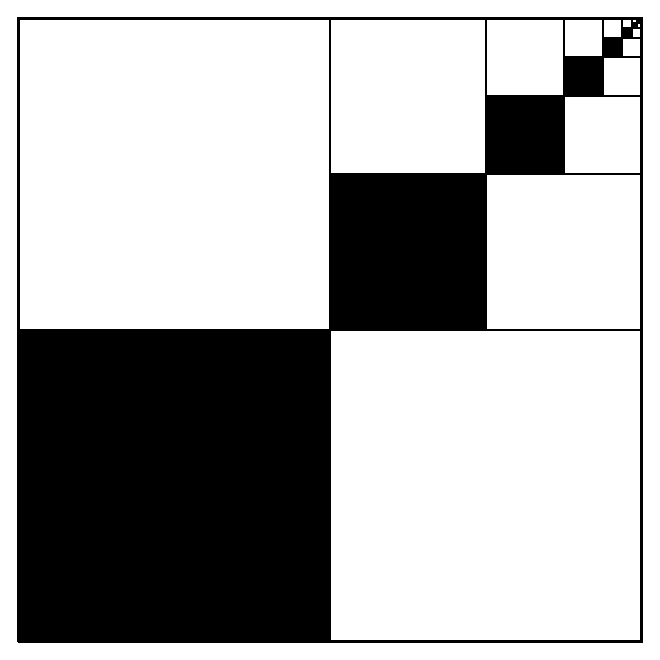
\includegraphics[width=300pt]{ChapterSeqSer/Figures/archimedessquare.eps}
	\end{center}

\vspace*{.1in}

Assume the entire square has side length 1 and that each further subdivision into squares uses side lengths that are half the previous.  

\begin{itemize}

\item What proportion of the whole large square is colored black?  As a consequence, what is the total area of all the black squares added up?

\vspace*{.5in}

\item Write the area of each individual black square and build an infinite series that represents the total black area.

\vspace*{.5in}

\item Find the sum of the series using the Geometric Series Formula. Verify it agrees with your total for the area above.

\vspace*{.5in}

\item Can you show the series converges using the No Hope Test?

\vspace*{.5in}

\item Can you show the series converges using the Geometric Series Test?

\vspace*{.5in}

\item Can you show the series converges using the Ratio Test?

\vspace*{.5in}

\item Can you show the series converges using the Alternating Series Test?

\vspace*{.5in}

\item Can you show the series converges using the Limit Comparison Test? 

\vspace*{.5in}

\item Can you show that the series converges using the Integral Test?

\vspace*{.5in}

\end{itemize}
\AnswerKeyEntry{The black region is one-third of the total square and thus must total to one-third.  The infinite series for the black square areas is $\frac{1}{4}+\frac{1}{16}+\frac{1}{32}+\frac{1}{64}+\cdots$.  NHT and AST give no information here, but all the rest of the tests work to determine convergence!  Use $\frac{1}{n^2}$ as a comparison function for LCT.}
\end{exercise}
